
\subsection{Choix des technologies et outils}
% Expliquer les choix technologiques (Node.js, Vue.js, React.js, PostgreSQL, etc.)
% Justifier ces choix en fonction des besoins du projet

Dans cette section, nous présentons les principales technologies utilisées pour le développement du projet. Chaque technologie a été sélectionnée pour ses performances, sa robustesse et sa facilité d’intégration dans notre stack.

\vspace{1cm} % Ajoute un espace vertical


\begin{longtable}{|m{4cm}|m{10cm}|}
    \hline
    \textbf{Technologie} & \textbf{Description} \\
    \hline
    \endfirsthead

    \hline
    \textbf{Technologie} & \textbf{Description} \\
    \hline
    \endhead

    \hline
    \endfoot

    \hline
    
\includegraphics[width=3cm]{images/logo/laravel.png} & 
    \textbf{Laravel - Framework Backend} : Laravel est un framework PHP moderne basé sur l’architecture MVC (Modèle-Vue-Contrôleur). Il offre de nombreuses fonctionnalités telles que :  
    \begin{itemize}
        \item Un ORM puissant (Eloquent) pour la gestion de la base de données.
        \item Un système de migration et de seeders pour faciliter le développement.
        \item Un mécanisme de routage avancé et un middleware intégré pour la gestion des requêtes HTTP.
    \end{itemize}
    Grâce à Laravel, nous avons pu structurer le projet de manière efficace et évolutive. \\
    \hline

    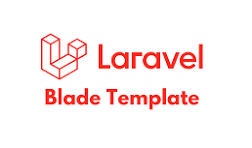
\includegraphics[width=3cm]{images/logo/blade.png} & 
    \textbf{Blade - Moteur de Templating} : Blade est le moteur de templates natif de Laravel. Il permet de créer des vues dynamiques avec une syntaxe claire et fluide. Ses principales caractéristiques sont :
    \begin{itemize}
        \item Une syntaxe simplifiée pour l'affichage des données et les structures de contrôle (`@if`, `@foreach`, etc.).
        \item La possibilité d’étendre des layouts grâce à l’héritage de templates.
        \item Une mise en cache automatique pour améliorer les performances.
    \end{itemize}\\
    \hline

    
\includegraphics[width=3cm]{images/logo/postgresql.png} & 
    \textbf{PostgreSQL - Base de Données Relationnelle} : PostgreSQL est un système de gestion de base de données relationnelle open-source reconnu pour sa stabilité et ses performances. Il a été choisi pour :  
    \begin{itemize}
        \item Son support avancé des types de données et des transactions ACID.
        \item Sa capacité à gérer de gros volumes de données efficacement.
        \item Son intégration facile avec Laravel via l'ORM Eloquent.
    \end{itemize}\\
    \hline

    
\includegraphics[width=3cm]{images/logo/bootstrap.png} & 
    \textbf{Bootstrap - Framework CSS} : Bootstrap est un framework CSS populaire utilisé pour concevoir une interface utilisateur réactive et attrayante. Il nous a permis de :  
    \begin{itemize}
        \item Utiliser un système de grille pour une mise en page responsive.
        \item Accélérer le développement avec des composants préconçus (modals, boutons, alertes, etc.).
        \item Assurer une compatibilité avec tous les navigateurs modernes.
    \end{itemize}\\
    \hline

    
\includegraphics[width=3cm]{images/logo/javascript.png} & 
    \textbf{JavaScript - Langage de Programmation Frontend} : JavaScript est un langage de programmation utilisé pour ajouter des interactions dynamiques à l'interface utilisateur. Il a été employé pour :  
    \begin{itemize}
        \item Gérer les interactions utilisateur (événements, animations).
        \item Améliorer l'expérience avec des requêtes asynchrones (AJAX, Fetch API).
        \item Dynamiser le rendu des composants sans recharger la page.
    \end{itemize}\\
    \hline

    
\includegraphics[width=3cm]{images/logo/git.png}  
    
\includegraphics[width=3cm]{images/logo/github.png} & 
    \textbf{Git et GitHub - Outils de Gestion de Version} : Pour la gestion du code source, nous avons utilisé **Git** et **GitHub** :  
    \begin{itemize}
        \item **Git** permet de suivre l'évolution du projet grâce à un système de versionnement performant.
        \item **GitHub** facilite la collaboration et l’hébergement du code en ligne, avec des fonctionnalités comme les pull requests et les issues.
    \end{itemize}
    Ces outils nous ont permis de travailler efficacement en équipe et d’assurer la stabilité du code tout au long du développement.\\
    \hline

\end{longtable}
\begin{center}  
    \captionof{table}{Tableau des technologies utilisées pour la réalisation} % Ajoute la légende à la liste des tableaux  
    \label{tab:table_techs_realisation} % Permet de faire référence à ce tableau plus tard
\end{center}  
L’utilisation de ces technologies nous a permis de construire une application performante, maintenable et évolutive. Le choix de Laravel avec Blade pour le backend, PostgreSQL pour la base de données et Bootstrap avec JavaScript pour le frontend a facilité l’implémentation et l’optimisation du projet. Enfin, l’utilisation de Git et GitHub a renforcé la gestion du code et le travail collaboratif.

%===========================================================================================================
